\subsection{One dimensional hydrogen chain}
\label{subsection:1dhydrogen}
We now move on to one of the simplest extended \emph{ab-initio} systems, a hydrogen chain in one dimension with periodic boundary conditions. 
We consider the case of $10$ atoms and work in a regime where the inter-atomic distance $r$ is 
relatively large ($r=1.5$ to $3.0$ \AA), such that the system is potentially well described by a one-band Hubbard model 
in terms of primarily $s$-like orbitals. 

For a given $r$, we first obtain single-particle Kohn-Sham orbitals from a set of spin-unrestricted and 
spin-restricted DFT-PBE calculations. The localized orbital basis upon which the RDMs (descriptors) 
are evaluated is obtained by generating intrinsic atomic orbitals (IAO) from the Kohn-Sham orbitals 
orthogonalized using the L\"owdin procedure. These are the orbitals that enter the one-band Hubbard Hamiltonian. 
Then, to generate a database of wavefunctions needed for the DMD, we produce a set of Slater-Jastrow 
wavefunctions consisting of singles- and doubles- excitations to the Slater determinant, 
\begin{subequations}
\begin{eqnarray}
| s \rangle = & e^J \Big[a^\dagger_{i \eta} a_{k \eta}   | KS \rangle \Big] \,,\\
| d \rangle = & \: e^J \Big[a^\dagger_{i \eta} a^\dagger_{j \eta'} a_{k \eta'} a_{l \eta}   | KS \rangle\Big] ,
\end{eqnarray}
\end{subequations}
where $|KS\rangle$ is the Slater determinant of occupied Kohn-Sham orbitals, $\eta$ and $\eta'$ are spin indices, 
and $a_{i}^\dagger$ ($a_{i}$) is a single-electron creation (destruction) operator corresponding to a particular Kohn-Sham orbital. $e^J$ is a Jastrow factor, optimized by minimizing the variance of the local energy. 
We compute the energies (expectation values of the Hamiltonian) and the RDMs on all the wave functions within Diffusion Monte Carlo (DMC). 
By computing the trace of the resulting 1-RDMs, we verify that all the electrons present in the system are represented within the localized basis of $s$-like orbitals. If the trace of the 1-RDM falls below the nominal number of electrons for a particular state, it 
indicates that some higher-energy orbitals are occupied ($p$-like orbitals, in the case of hydrogen), and that the state can not be described by the low-energy model Hamiltonian. We exclude such states from further analysis. The acquired data set is then used in DMD to 
downfold to a one-band Hubbard Hamiltonian.% described in Sec. \ref{sec:theory}.

\begin{figure}
\centering
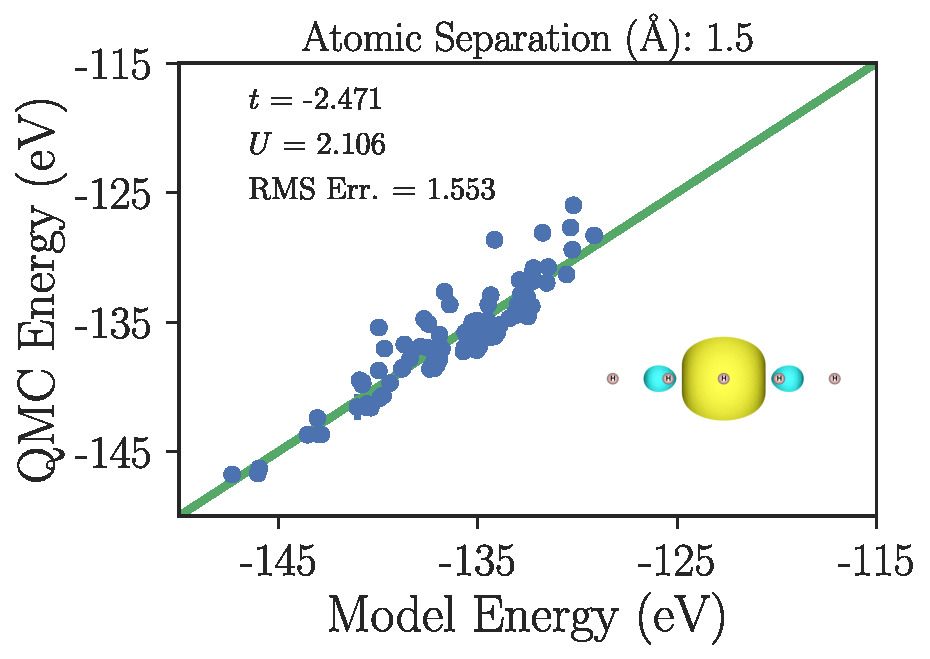
\includegraphics[scale=0.32]{{./Figures/H_chain_fit_model_length1.5_tUs_inset}.eps}
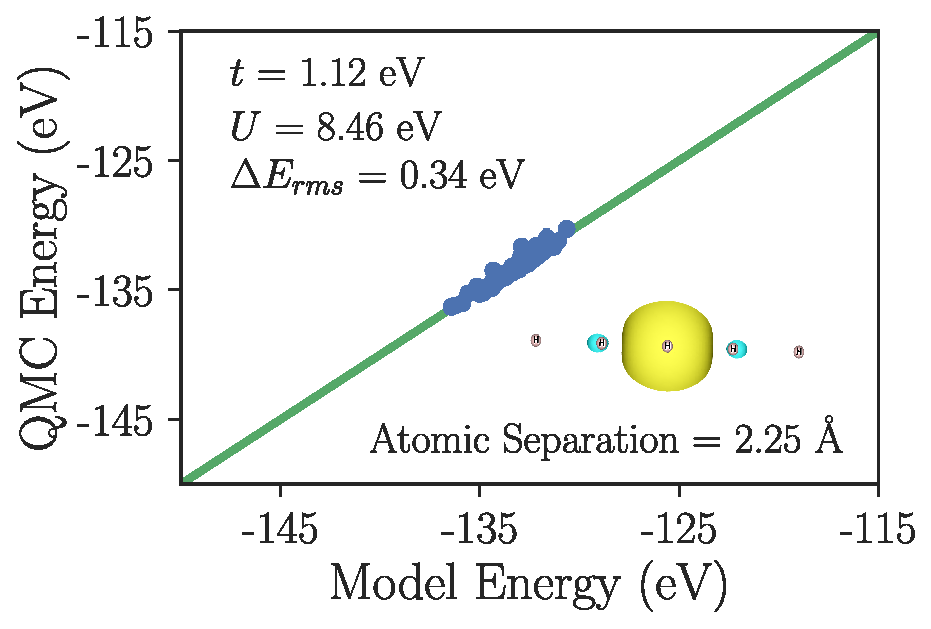
\includegraphics[scale=0.32]{{./Figures/H_chain_fit_model_length2.25_tUs_inset}.eps}
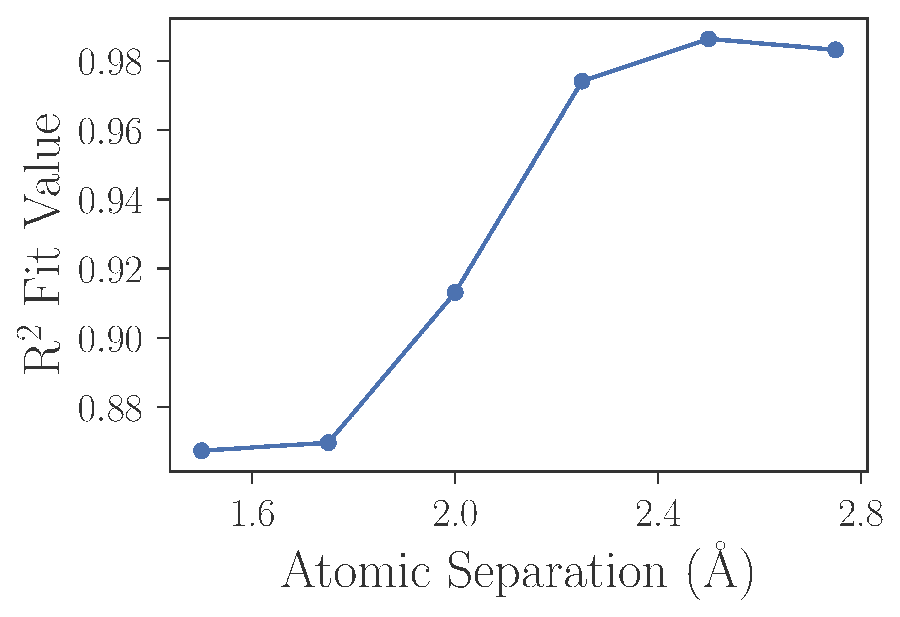
\includegraphics[scale=0.32]{{./Figures/r2_ut_vs_separation_h_chain}.eps}
\caption{Diffusion Monte Carlo energy versus the reconstructed 
model energy for the H$_{10}$ chain at (A) 1.5 \AA \: and (B) 2.25 \AA \:. The energy range of excitations 
narrows significantly for larger interatomic separation. Insets show the intrinsic atomic orbitals which constitute the one-body space 
which was used for calculating the reduced density matrices (descriptors).
}
\label{fig:fit_quality}
\end{figure}

Fig.~\ref{fig:fit_quality} shows our DMD fits for two representative $r$. The model energy is the energy 
reconstructed from the optimized parameters $t$ and $U$ and the RDMs. For $r=1.5$ \AA \:, there is 
considerable spread in the data from the 45 degree line indicating that the simple short range Hubbard model 
is insufficient for an \textit{accurate} description in the corresponding energy window. 
In contrast, the root mean square (RMS) error is significantly smaller for larger $r$, suggesting the increased 
effectiveness of the one-band Hubbard model. The insets show the intrinsic atomic orbitals for which we calculated 
the RDMs (descriptors). 

\begin{figure}
\centering
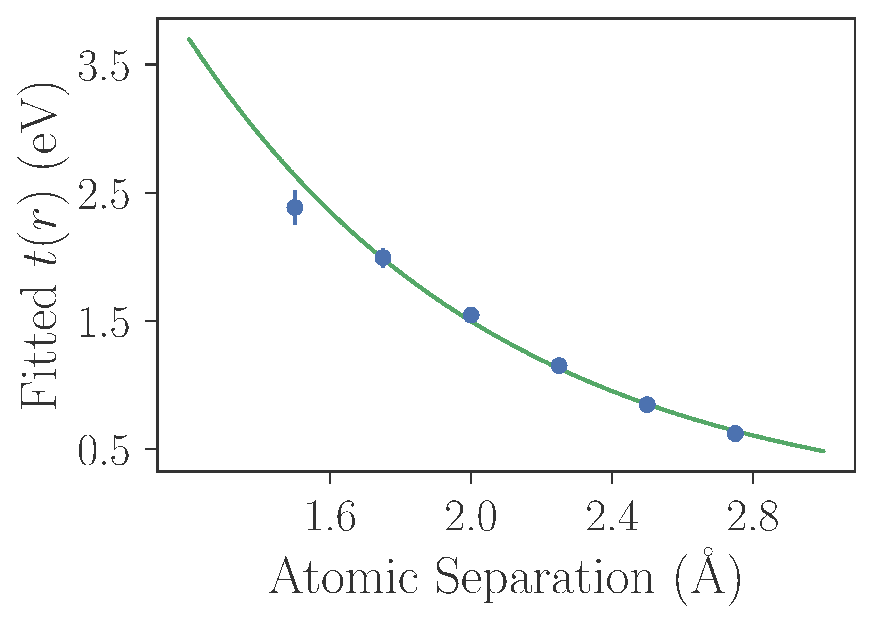
\includegraphics[scale=0.5]{./Figures/fitted_t_values_no_offset_h10_chain.eps}
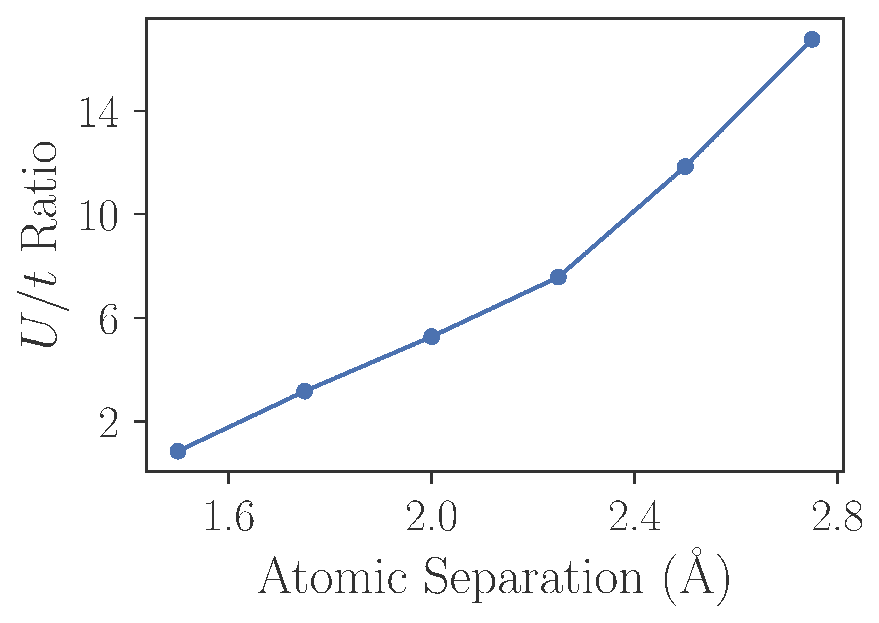
\includegraphics[scale=0.5]{./Figures/Ust_ratio_vs_separation_h_chain.eps}
\caption{(Left) The one-body hopping $t$ parameter as a function of interatomic distance for the periodic H$_{10}$ chain, obtained from a fitted $U$-$t$ model. $t$ declines to zero as $r$ increases. (Right) The ratio $U/t$ for the fitted parameter values as a function of interatomic separation. The ratio is small at lower bond-lengths, where $t$ is more relevant in describing the system, and larger at longer bond-lengths, where inter-site hopping is less significant. }\label{fig:Parameters-vs-Bond-t}
\end{figure}

Fig.~\ref{fig:Parameters-vs-Bond-t} shows trends of the DMD values of $t$ and $U$ as a function of $r$. 
Consistent with physical intuition, $t$ decreases towards zero at larger $r$
and the value of $U/t$ rises. However, as previously mentioned, the single-band 
Hubbard model is not expected to describe the hydrogen chain well at small distances. 
The one dimensional Hubbard model with $U/t>0$ will always result in 
an Mott insulating state. In comparison, for the idealized hydrogen chain, the 
metal-to-insulator transition has been shown to occur at $r_c \sim 1.8$\AA~\cite{Stella2011}, which would correspond 
to a finite non-zero $U$. This indicates that at small distance, the higher energy orbitals play a nontrivial 
role in stabilizing the metallic state of hydrogen, instead of merely renormalizing the effective strength of $U$. 
At small distances, other interactions like nearest neighbor Coulomb 
and exchange interactions also become important for $r<r_c$ \cite{ZhengThesis}. 
